% !TEX root = /home/computer/ucsc/master-2/quarter-2/numerical-linear-algebra/master.tex
\assignment{1}{Sat 29 Jan 2022 15:42}{Assignment 1}

\subsectionfont{\fontsize{10}{10}\selectfont}

\graphicspath{{./assignment_01/figures/}}

\section{Problem 1}%
\label{sec:problem_1}
\subsection{If $A\in\C$ is unitary and upper triangular, then $A$ is diagonal}%
\label{sub:1.1}

$A\in\C^{m\times m}$ unitary implies, by definition,

\[
  A^{*}A = AA^{*} = I
.\] 

If $A$ is upper triangular, then 

\begin{align*}
  A^{*}A &= \begin{pmatrix}
              \overline{a_{11}} & 0 & \hdots & 0  \\
              \overline{a_{12}} & \overline{a_{22}} & \hdots & 0 \\
              \vdots & \vdots & \ddots & \vdots \\
              \overline{a_{1m}} & \overline{a_{2m}} & \hdots & \overline{a_{mm}}
            \end{pmatrix} 
            \begin{pmatrix}
               a_{11} & a_{12} & \dots & a_{1m} \\
               0 & a_{22} & \dots & a_{2m} \\
               \vdots & \vdots & \ddots & \vdots \\
               0 & 0 & \dots & a_{mm} \\
            \end{pmatrix} \\
\end{align*}

where $\overline{a_{ij}}$ is the conjugate of $a_{ij}$. Then the first column of
$A^{*}A=\bm{e_1}$, where $\bm{e_1}$ is the standard basis vector,
 \[
  \begin{pmatrix}
    \overline{a_{11}} & 0 & \hdots & 0  \\
    \overline{a_{12}} & \overline{a_{22}} & \hdots & 0 \\
    \vdots & \vdots & \ddots & \vdots \\
    \overline{a_{1m}} & \overline{a_{2m}} & \hdots & \overline{a_{mm}}
  \end{pmatrix}
  \begin{pmatrix} a_{11} \\ 0 \\ \vdots \\ 0 \end{pmatrix} = \bm{e_1}
.\] 

implies $|a_{11}|^2 = 1$, and
\[
\overline{a_{1j}} = a_{1j} = 0 \qquad \text{for } j > i = 1
.\] 

Continuing for the remaining columns, we find that $|a_{ii}|^2=1$ and
\[
\overline{a_{ij}} = a_{ij} = 0 \qquad \text{for } j > i = 2, 3, \dots, m
.\] 

This implies that $A$ is diagonal. This would also hold if $A$ is lower
triangular and unitary since, $A^{*}A = AA^{*}$. $\;\Box$. 

\section{Problem 2}%
\label{sec:problem_2}
\subsection{If $A$ is invertible and $\lambda \neq 0$ is an eigenvalue of $A$,
then $\frac{1}{\lambda }$ is an eigenvalue of $A^{-1}$}%
\label{sub:2.1}

Let $\left(\lambda, v\right)$ be an eigenpair for $A\in \mathbb{C}$, then
\begin{align*}
  Av &= \lambda v \\
  A^{-1} Av &= \lambda A^{-1}v && \text{multiplying by } A^{-1} \\
  \frac{1}{\lambda}v &= A^{-1}v \\
\end{align*}
$\implies \frac{1}{\lambda} \text{ is an eigenvalue of $A^{-1}$}$, and
$A$ and  $A^{-1}$ have the same eigenvectors. $\Box$

\subsection{Show $AB=BA$ have the same eigenvalues.}%
\label{sub:2.2}
Let $Bv = w$ and $ (\lambda ,v)$ be an eigenpair of $AB$, then
\begin{align*}
  \left(AB\right)v &= \lambda v
\end{align*}

implies
\[
Aw = \lambda v
.\] 

Multiplying both sides by $B$ 

\begin{align*}
    \left(BA\right)w &= \lambda Bv \\
          &= \lambda w
\end{align*}

$\implies$ $\lambda$ is an eigenvalue of both $AB$ and $BA$ with different
eigenvectors. $\Box$

\subsection{Show $A\in\R$ and $A^{*}$ have the same eigenvalues}%
\label{sub:2.3}

Let $\langle \cdot, \cdot \rangle$ be an inner
product, and $(\lambda,v)$ be an eigenpair of  $A$, then
\begin{align*}
  \langle Av,Av \rangle &= \lambda  \langle v, Av \rangle \\
  &= \lambda \bar\lambda\langle  v, v \rangle \quad
  \text{conjugate linearity} \\
  &= \lambda \langle A^{*}v, v \rangle \quad \text{definition of adjoint}
\end{align*}
$\implies A^{*}v = \bar \lambda v$. So $(\bar\lambda,v) $ is an eigenpair of
$A^{*}$, and since complex eigenvalues of a real valued matrix come in conjugate
pairs then both  $\lambda $ and $\bar \lambda $ are eigenvalues of $A$ and
$A^{*}$. Otherwise if $\lambda \in\R$, then $\lambda = \bar \lambda $, and
hence they have the same eigenvalues. $\Box$

\section{Problem 3}%
\label{sec:problem_3}

\textbf{Let $A\in\C$ be hermitian} 

\subsection{ Prove all eigenvalues of $A$ are real}%
\label{sub:3.1}

\[
\langle Av,v\rangle =\lambda\langle
v,v\rangle\underbrace{=}_{\text{definition of Adjoint}} \langle v,
A^*v\rangle \underbrace{=}_{\text{$A$ hermitian}} \langle v,Av\rangle
\underbrace{=}_{\text{conjugate symmetry}} \bar\lambda\langle v,v\rangle
.\] 

$\implies \lambda =\bar\lambda\implies\lambda\in\mathbb{R}$
Since the only way $\lambda$ equals its conjugate is if it is real.


\subsection{If $x$ and $y$ are eigenvectors corresponding to distinct
eigenvalues, show they are orthogonal}%
\label{sub:3.2}


\[
\langle Ax, y \rangle = \lambda_x\langle x, y\rangle
  \underbrace{=}_{\text{Hermitian}} \langle x,
Ay \rangle \underbrace{=}_{\text{$\lambda_y\in\mathbb{R}$}} \lambda_y \langle x,y\rangle
.\] 
$\text{Since } \lambda_x \neq\lambda_y \text{ (distinct)}$, then $\langle x, y\rangle= 0$ 

\section{Problem 4}%
\label{sec:problem_4}

\textbf{Show that a hermitian matrix $A$ is positive definite iff $\lambda
_{i}>0$ for all $\lambda _{i}$ in the spectrum of $A$} 

Since $A$ is hermitian, then $A$ is unitarily diagonalizable with real
eigenvalues, i.e. $A = UDU^{*}$ where $D$ is diagonal and $U$ is unitary,
$ (U^{*}U = I)$. Considering change of basis $y = U^{*}x$ into the basis where
$A$ is diagonal, then $y^{*} = x^{*}U$ and
\begin{align*}
  \langle Ax,x \rangle &= \langle UDU^{*}x,x \rangle \\
                       &= y^{*}Dy \\
                       &= \sum^{m}_{i=1} \lambda _{i}y^{*}y \\
                       &= \sum^{m}_{i=1} \lambda _{i}\|y\|^{2} \\
\end{align*}

Since $\|y\|^{2} > 0$ for $x \neq 0$, then $ \langle Ax,x \rangle > 0 $ if and
only if $\lambda _{i} > 0$

\section{Problem 5}%
\label{sec:problem_5}

\textbf{Let $A\in\C$ be unitary} 

\subsection{Let $ (\lambda, x)$ be an eigenpair of $A$, show $|\lambda | = 1$}%
\label{sub:5.1}
$A$ unitary implies $A^{*}A = I$
\[
\langle Av,Av\rangle = \lambda\bar\lambda\langle v,v\rangle
= |\lambda|^2 \langle v, v\rangle = \langle v,A^*Av\rangle = \langle
v ,v\rangle
.\] 
$\implies |\lambda| = 1$ 

\subsection{Prove or disprove $\|A\|_{F} = 1$}%
\label{sub:5.2}

\[
\|A\|_F^2=Tr(A^*A)=Tr(I)=m\neq1
.\] 


\section{Problem 6}%
\label{sec:problem_6}

\textbf{Let $A\in\C$ be skew-hermition} 

\subsection{Show eigenvalues of $A$ are pure imaginary}%
\label{sub:6.1}

\[
\langle Av,v\rangle = \underbrace{\lambda \langle
  v,v\rangle} = \langle
  v, A^*\rangle = \langle v, -Av\rangle = \underbrace{-\bar\lambda \langle v,
  v\rangle}
.\] 

$ \implies \lambda = -\bar \lambda \implies \lambda\in\mathbb{C}$ is pure
imaginary

 \subsection{Show $I-A$ is nonsingular}%
\label{sub:6.2}
Consider $v\in \ker(I-A)$
\begin{align*}
  (I-A)v&=0 \\
  Iv =v &=Av 
\end{align*}
Then,
\[
\langle v,v\rangle = \langle Av, v\rangle = \langle v, A^*v\rangle
= -\langle v,v\rangle
.\] 
Which is only possible if $v=0$. This shows the kernal is trivial,
and hence $I-A$ is nonsingular.


\section{Problem 7}%
\label{sec:problem_7}
\textbf{Show $ \rho (A) \leq \|A\|$, where $\rho (A)$ is the spectral radius of $A$} 

  Spectral radius $\rho (A) =\max{\left\{|
    \lambda_1|,|\lambda_2|, \dots, |\lambda_n|\right\}}$.

    \begin{align*}
      \|Ax\|^2 = \langle Ax,Ax\rangle &= \lambda\bar \lambda \langle x,
      x\rangle \\
      &= | \lambda|^2 \cancel{\|x\|^2} \underbrace{\leq}_{\text{property of
      induced norm}} = \|A\|^2\cancel{\|x\|^2}
    \end{align*}
$\implies |\lambda| \leq \|A\|$  $\forall \lambda$ $\implies \rho(A) \leq
\|A\|$


\section{Problem 8}%
\label{sec:problem_8}

\textbf{Let $A$ be defined by the inner product $A = uv^{*}$} 

\subsection{Prove of disprove $\|A\|_{2} = \|u\|_{2}\|v\|_{2}$}%
\label{sub:prove_of_disprove_|a|__2_|u|__2_$}

Consider $A^{*}Av$ 
\begin{align*}
  A^*Av&=vu^*uv^*v \\
       &=\|u\|_2^2v(v^*v) \\
       &=\|u\|_2^2\|v\|_2^2v
\end{align*}

This shows $v$ is the only eigenvector of $A^{*}A$, and since $A$ is rank 1, this is the only singular value (squared). So

\[
\implies \|A\|_2=\sigma_{\max{}}=\sigma=\|u\|_2\|v\|_2
.\] 

\subsection{Prove or disprove $\|A\|_F=\|u\|_F\|v\|_F$}%
\label{sub:8.2}
Since $A$ is rank $1$ the equality holds. Where the only singular value of $A$ is
          $\sigma = \|u\|_2\|v\|_2$. Since, the frobenius norm is the same as the
          two norm for vectors, then
\[
  \|A\|_F = \sqrt{Tr(A^*A)} = \sum^m_{i=1}\sqrt{\sigma_i^2} = \sigma
  = \|u\|_2\|v\|_2=\|u\|_F\|v\|_F = \|A\|_2
.\] 

\section{Problem 9}%
\label{sec:problem_9}

\textbf{$A, Q\in\C$ where $A$ is arbitrary and Q is unitary} 

\subsection{Show $\|AQ\|_{2} = \|A\|_{2}$}%
\label{sub:9.1$}

Definition of $2$-norm, and $Q$ unitary, its easy to see that $\|QA\|_{2}$

\[
  \|QA\|_{2} = \sqrt{\lambda _{\text{max}} (A^{*}Q^{*}QA)} = \sqrt{\lambda
_{\text{max}} (A^{*}A)} = \sigma_{\text{max}} (A) = \|A\|_{2}
.\] 

If we let $B = QA$, then noting that  $B*B$, and $BB^{*}$ are positive definite
\begin{align*}
  \langle B^{*}Bx, x \rangle &= \langle Bx,Bx \rangle > 0 \\
  \langle BB^{*}x, x \rangle & = \langle B^{*}x, B^{*}x \rangle > 0
\end{align*}

for $x \neq 0$, then referencing problem (\ref{sub:10.1})

  \begin{align*}
    \|AQ\|_{2} = \sqrt{\lambda _{\text{max}} (Q^{*}A^{*}AQ)} = \sqrt{\lambda
    _{\text{max}} (B^{*}B)} &= \sigma_{\text{max}} (B^{*}B) \\
                            &= \sigma_{\text{max}} (BB^{*}) \\
                            &= \|AQ\|_{2} \\
                            &= \|A\|_{2}
  \end{align*}

\subsection{Show $\|AQ\|_{F} = \|QA\|_{F} = \|A\|_{F}$ }%
\label{sub:10.2}

First it's easy to show $\|QA\|_{F} = \|A\|_{F}$
\[
  \|QA\|_{F} = \sqrt{ \text{trace}(A^{*}Q^{*}QA)} =\sqrt{ \text{trace}(A^{*}A)}
  = \|A\|_{F}
.\] 

then using the cyclic nature of the trace

\[
  \|AQ\|_{F} = \sqrt{ \text{trace}(Q^{*}A^{*}AQ)} =\sqrt{ \text{trace}(QQ^{*}A^{*}A)}
   \sqrt{ \text{trace}(A^{*}A)} = \|A\|_{F}
.\] 


\section{Problem 10}%
\label{sec:problem_10}

\subsection{Show that if $A$ and $B$ are unitarily equivalent, then they have
the same singular values.}%
\label{sub:10.1}
Unitarily equivalent means $A = QBQ^{*}$ for some unitary $Q\in\C$.

Since $A$ is square and has SVD, write $A=U\Sigma V^*$. Then.
  \begin{align*}
    A = U\Sigma V^* &= QBQ^* \\
    Q^*U\Sigma V^*Q &= B \\
    \hat U\Sigma \hat V^* &= B
  \end{align*}

  Which forms the SVD of $B$. Hence $A$ and $B$ have the same singular
  values. This can be seen by noting $\hat U$ and $\hat V$ form the
  unitary eigendecomposition of  $BB^*$ and $B^*B$ respectively. i.e.

  \begin{align*}
    BB^* &= Q^*U\Sigma^2U^*Q \\
         &= \hat U\Sigma^2\hat U^* && \text{and,} \\
    B^*B &= Q^*V\Sigma^2V^*Q \\
         &= \hat V\Sigma^2\hat V^*
  \end{align*}

\subsection{Show the converse is not necessarily true}%
\label{sub:10.2}

\section{Problem 11}%
\label{sec:problem_11}

\textbf{Find the relative condition number of the following functions and discuss if there is any concern of being ill-conditioned} 

\subsection{$f (x_1,x_2) = x_1 + x_2$}%
\label{sub:11.1}

The Jacobian is  $Jf= \begin{pmatrix} 1 && 1 \end{pmatrix}$. Using the infinity norm the relative condition number is

\[
  \kappa = \frac{\|Jf(x)\|_\infty\|x\|_\infty}{\|f(x)\|_\infty}
= \frac{2\max{\{|x_1|,|x_2|\}}}{|x_1+x_2|}
.\] 
This is ill-conditioned for $x_1\longrightarrow -x_2$

\subsection{$f (x_1,x_2) = x_1 x_2$}%
\label{sub:11.2}

The Jacobian is  $Jf= \left(\begin{matrix} x_2 && x_1 \end{matrix}
\right)$. Using the infinity norm the relative condition number is.
\[
  \kappa = \frac{\|Jf(x)\|_\infty\|x\|_\infty}{\|f(x)\|_\infty}
= \frac{ \left(|x_2|+|x_1|\right)\max{\{|x_1|,|x_2|\}}}{|x_1x_2|}
.\] 
This is ill-conditioned for $x_1\text{ or } x_2\longrightarrow 0$

\subsection{$f (x) = (x-2)^{9}$}%
\label{sub:11.2}
The Jacobian is  $Jf=9(x-2)^8$. Using the
          infinity norm, the relative condition number is.
          \begin{align*}
            \kappa &= \frac{|9(x-2)^8||x|}{|(x-2)^9|} \\
                   &= \frac{|9x|}{|x-2|} \frac{|x+2|}{|x+2|} \\
                   & = \frac{|9x^2+ 18x|}{x^2+4}
          \end{align*}
Which, after simplifying, we see is not ill-conditioned.

\section{Problem 12}%
\label{sec:problem_12}

\subsection{Plot $f(x)$}%
\label{sub:12.1}

\begin{figure}[H]
  \centering
  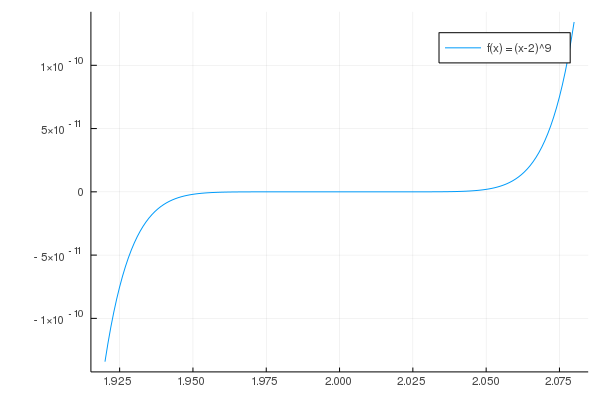
\includegraphics[width=0.8\linewidth]{plot_a.png}
  \caption{Plot f}%
  \label{fig:plota}
\end{figure}

\subsection{Plot $g(x)$}%
\label{sub:12.2}

\begin{figure}[H]
  \centering
  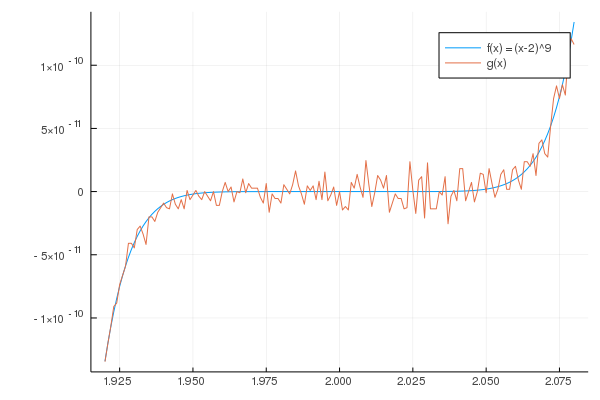
\includegraphics[width=0.8\linewidth]{plot_b.png}
  \caption{Plot f and g}%
  \label{fig:plotb}
\end{figure}

\subsection{Conclusion}%
\label{sub:12.3}

It appears the expanded form of $g(x)$ is unable to remove the discontinuity at
$x = 2$
